\chapter{Appendix}

\printglossaries

\newpage

\section{LiveInfoLogger Data Fields}
\label{des:liveinfodatafields}

The following fields are currently available in the LiveInfo data file, which contains information about the simulation state at each iteration. The data is collected and logged by the \texttt{LiveInfoLogger} class of the \gls{autopas} library.

\begin{description}[style=multiline, leftmargin =40mm]
    \item [Iteration] The current iteration number of the simulation.
    \item [avgParticlesPerCell] The average number of particles per cell in the simulation domain.
    \item [cutoff] The cutoff radius for the interaction of particles, beyond which particles do not interact.
    \item [domainSizeX] The size of the simulation domain in the X dimension.
    \item [domainSizeY] The size of the simulation domain in the Y dimension.
    \item [domainSizeZ] The size of the simulation domain in the Z dimension.
    \item [estimatedNumNeighborInteractions] The estimated number of neighbor interactions between particles.
    \item [homogeneity] A measure of the distribution uniformity of particles across the cells. \todo{Define the metric}
    \item [maxDensity] The maximum density of particles in any cell.
    \item [maxParticlesPerCell] The maximum number of particles found in any single cell.
    \item [minParticlesPerCell] The minimum number of particles found in any single cell.
    \item [numCells] The total number of cells in the simulation domain.
    \item [numEmptyCells] The number of cells that contain no particles.
    \item [numHaloParticles] The number of particles in the halo region (boundary region) of the simulation domain.
    \item [numParticles] The total number of particles in the simulation domain.
    \item [particleSize] The size of each particle. \todo{Which unit?}
    \item [particleSizeNeededByFunctor] The particle size required by the functor (the function used for calculating interactions).
    \item [particlesPerBlurredCellStdDev] The standard deviation of the number of particles per blurred cell, providing a measure of particle distribution variability.
    \item [particlesPerCellStdDev] The standard deviation of the number of particles per cell, indicating the variability in particle distribution.
    \item [rebuildFrequency] The frequency at which the neighbor list is rebuilt.
    \item [skin] The skin width added to the cutoff radius to create a buffer zone for neighbor lists, ensuring efficient interaction calculations.
    \item [threadCount] The number of threads used for parallel processing in the simulation.
\end{description}


\section{TuninData Fields}
\label{des:tuningdatafields}

The following fields are currently available in the TuningResults data file, which contains the current performance data for a given configuration at a particular iteration. The data is collected and logged by the \texttt{TuningDataLogger} class of the \gls{autopas} library.

\begin{description}[style=multiline, leftmargin =40mm]
    \item[Date] The date and time when the data was collected.
    \item[Iteration] The current iteration number of the simulation.
    \item[Container] The type of container used to store the particles in the simulation (e.g., LinkedCells, VerletLists).
    \item[CellSizeFactor] A factor that determines the size of the cells relative to the cutoff radius. \todo{check https://mediatum.ub.tum.de/doc/1518839/1518839.pdf}
    \item[Traversal] The method used to traverse the cells and calculate interactions between particles.
    \item[Load Estimator] The strategy used to estimate and balance the computational load across different parts of the simulation domain.
    \item[Data Layout] The arrangement of particle data in memory (e.g., AoS for Array of Structures, SoA for Structure of Arrays).
    \item[Newton 3] Indicates whether the Newton's third law optimization is used to reduce computation by only calculating forces once per particle pair (Yes/No).
    \item[sample$i$] The performance data for the configuration at the $i$-th sample point. The number of total sample points per iteration can be configured via the \texttt{.yaml} configuration file.
    \item[Reduced] The reduced performance data for all sample points, calculated by aggregating the data across all sample points. The specific aggregation method can be configured via the \texttt{.yaml} configuration file.
    \item[Smoothed] A smoothed version of the reduced performance data.

\end{description}


\section{ANTLR4 Rule Parser Grammar}

The following is the grammar for the domain-specific language used by the Rule Parser to parse the rule base supplied by the user. The grammar is defined using the ANTLR4 parser generator.


\lstset{
    backgroundcolor=\color{gray!10},
    framexleftmargin=5pt,
    framextopmargin=5pt,
    numbers=left,
}%

% Applies only when you use it
\lstdefinestyle{MyLang}{
    basicstyle=\small\ttfamily,%
    breaklines=true,%                                      
    moredelim=[s][\color{green!50!black}\ttfamily]{'}{'},
    commentstyle={\color{gray}\itshape},%                  
    morecomment=[l]{//},
    morekeywords={rule_file, settings, linguistic_variable, fuzzy_term, function, fuzzy_rule, fuzzy_set, output_mapping, output_entry, pattern_mapping, config_pattern},
    keywordstyle={\color{red!90!black!70}\bfseries},%
    emph={STRING, NUMBER, IDENTIFIER, WS, COMMENT, INT, EXP, EOF},
    emphstyle={\color{blue}\ttfamily},
}


\begin{lstlisting}[style=MyLang,basicstyle=\tiny, caption={ANTLR4 Rule Parser Grammar}, label={lst:antlr4grammar}]
grammar FuzzyLanguage;

// Rule File
rule_file           : settings linguistic_variable* 
                      output_mapping fuzzy_rule* EOF
                    ;

// Settings as key-value pairs
settings            : 'FuzzySystemSettings' ':'
                    (IDENTIFIER ':' STRING)*
                    ;

// Fuzzy Variable
linguistic_variable
                    : 'FuzzyVariable' ':' 'domain' ':' STRING 
                        'range' ':' '(' NUMBER ',' NUMBER ')' 
                       fuzzy_term+
                    ;

fuzzy_term
                    : STRING ':' function
                    ;

function
                    : IDENTIFIER '(' NUMBER (',' NUMBER)* ')'
                    ;

// Fuzzy Rule
fuzzy_rule
                    : 'if' fuzzy_set 'then' fuzzy_set
                    ;

fuzzy_set
                    : '(' fuzzy_set ')'         # Brackets
                    | fuzzy_set '&&' fuzzy_set  # And
                    | fuzzy_set '||' fuzzy_set  # Or
                    | '!' fuzzy_set             # Negate
                    | STRING '==' STRING        # Select
                    ;

// Output Mapping
output_mapping
                    : 'OutputMapping' ':'
                       output_entry+
                    ;

output_entry
                    : STRING ':' pattern_mapping+
                    ;

pattern_mapping
                    : NUMBER '=>' 
                        config_pattern (',' config_pattern)*
                    ;

config_pattern
                    : '[' (IDENTIFIER '=' STRING) 
                          (',' IDENTIFIER '=' STRING)* ']'
                    ;

// Lexer Rules
WS
                    : [ \t\n\r\f]+ -> skip
                    ;

COMMENT             : '#' .*? '\r'? '\n' -> skip
                    ;

STRING
                    : '"' (~["\r\n] | '""')* '"'
                    {setText(getText().substr(1, getText().size()-2));}
                    ;

NUMBER
                    : '-'? INT ('.' [0-9]+)? EXP?
                    ;

fragment INT
                    : '0'
                    | [1-9] [0-9]*
                    ;

fragment EXP
                    : [Ee] [+-]? [0-9]+
                    ;

IDENTIFIER
                    : [a-zA-Z0-9_]+
                    ;
\end{lstlisting}

\section{Scenarios used for Data Generation}
\label{des:scenarios}

The following scenarios were used to generate the data to train the decision tree models used to generate the fuzzy rules. The scenarios are defined in the \texttt{.yaml} configuration file used by the \texttt{AutoPas} library.

\begin{lstlisting}[language=yaml,basicstyle=\tiny,breaklines=true,  caption={explodingLiquid.yaml}, label={lst:explodingLiquid}]
container                        :  [LinkedCells, VarVerletListsAsBuild, VerletClusterLists, VerletLists, VerletListsCells, PairwiseVerletLists]
verlet-rebuild-frequency         :  10
verlet-skin-radius-per-timestep  :  0.02
fastParticlesThrow               :  false
verlet-cluster-size              :  4
selector-strategy                :  Fastest-Mean-Value
data-layout                      :  [AoS, SoA]
traversal                        :  [lc_c01, lc_c01_combined_SoA, lc_c04, lc_c04_HCP, lc_c04_combined_SoA, lc_c08, lc_c18, lc_sliced, lc_sliced_balanced, lc_sliced_c02, vcl_c01_balanced, vcl_c06, vcl_sliced, vcl_sliced_balanced, vcl_sliced_c02, vl_list_iteration, vlc_c01, vlc_c18, vlc_sliced, vlc_sliced_balanced, vlc_sliced_c02, vlp_c01, vlp_c18, vlp_sliced, vlp_sliced_balanced, vlp_sliced_c02, vvl_as_built]
tuning-strategies                :  []
tuning-interval                  :  1000
tuning-samples                   :  10
functor                          :  Lennard-Jones (12-6) AVX intrinsics
newton3                          :  [disabled, enabled]
cutoff                           :  2
box-min                          :  [0, 0, 0]
box-max                          :  [15, 60, 15]
cell-size                        :  [1]
deltaT                           :  0.00182367
sorting-threshold                :  8
iterations                       :  12000
boundary-type                    :  [periodic, periodic, periodic]
Sites:                           
  0:
    epsilon                      :  1
    sigma                        :  1
    mass                         :  1
Objects:                         
  CubeClosestPacked:
    0:  
      particle-spacing           :  1
      box-length                 :  [14, 6, 14]
      bottomLeftCorner           :  [0.5, 27, 0.5]
      velocity                   :  [0, 0, 0]
      particle-type-id           :  0
vtk-filename                     :  explodingLiquid
vtk-write-frequency              :  10000000
use-tuning-logger                :  false
output-suffix                    :  
log-level                        :  info
no-flops                         :  false
no-end-config                    :  true
no-progress-bar                  :  false
load-balancer                    :  InvertedPressure
load-balancing-interval          :  100
subdivide-dimension              :  [true, true, true]
\end{lstlisting}

\begin{lstlisting}[language=yaml,basicstyle=\tiny,breaklines=true,  caption={spinodalDecompositionEquilibration.yaml}, label={lst:spinodalDecompositionEquilibration}]
container                        :  [LinkedCells, VerletClusterLists, VerletLists, VerletListsCells, PairwiseVerletLists]
verlet-rebuild-frequency         :  10
verlet-skin-radius-per-timestep  :  0.05
fastParticlesThrow               :  false
verlet-cluster-size              :  4
selector-strategy                :  Fastest-Absolute-Value
data-layout                      :  [AoS, SoA]
traversal                        :  [lc_c01, lc_c01_combined_SoA, lc_c04, lc_c04_HCP, lc_c04_combined_SoA, lc_c08, lc_c18, lc_sliced, lc_sliced_balanced, lc_sliced_c02, ot_c01, ot_c18, vcl_c01_balanced, vcl_c06, vcl_sliced, vcl_sliced_balanced, vcl_sliced_c02, vl_list_iteration, vlc_c01, vlc_c18, vlc_sliced, vlc_sliced_balanced, vlc_sliced_c02, vlp_c01, vlp_c18, vlp_sliced, vlp_sliced_balanced, vlp_sliced_c02, vlp_c08, vvl_as_built]
tuning-strategies                :  []
tuning-interval                  :  1000
tuning-samples                   :  3
functor                          :  Lennard-Jones (12-6) AVX intrinsics
newton3                          :  [disabled, enabled]
cutoff                           :  2.5
box-min                          :  [-0.25, -0.25, -0.25]
box-max                          :  [46, 46, 46]
cell-size                        :  [1]
deltaT                           :  0.00182367
sorting-threshold                :  8
iterations                       :  10000
boundary-type                    :  [periodic, periodic, periodic]
Sites:                           
    0:
    epsilon                      :  1
    sigma                        :  1
    mass                         :  1
Objects:                         
    CubeGrid:
    0:  
        particles-per-dimension  :  [30, 30, 30]
        particle-spacing         :  1.5
        bottomLeftCorner         :  [0.5, 0.5, 0.5]
        velocity                 :  [0, 0, 0]
        particle-type-id         :  0
thermostat:
    initialTemperature           :  1.4
    targetTemperature            :  1.4
    deltaTemperature             :  2
    thermostatInterval           :  10
    addBrownianMotion            :  true
vtk-filename                     :  SpinodalDecomposition_equilibration
vtk-write-frequency              :  10000
use-tuning-logger                :  false
output-suffix                    :  
log-level                        :  info
no-flops                         :  false
no-end-config                    :  false
no-progress-bar                  :  false
load-balancer                    :  InvertedPressure
load-balancing-interval          :  100
subdivide-dimension              :  [true, true, true]
\end{lstlisting}

\begin{lstlisting}[language=yaml,basicstyle=\tiny,breaklines=true,  caption={spinodalDecomposition.yaml}, label={lst:spinodalDecomposition}]
container                        :  [LinkedCells, VerletClusterLists, VerletLists, VerletListsCells, PairwiseVerletLists]
verlet-rebuild-frequency         :  15
verlet-skin-radius-per-timestep  :  0.2
fastParticlesThrow               :  false
verlet-cluster-size              :  4
selector-strategy                :  Fastest-Absolute-Value
data-layout                      :  [AoS, SoA]
traversal                        :  [lc_c01, lc_c01_combined_SoA, lc_c04, lc_c04_HCP, lc_c04_combined_SoA, lc_c08, lc_c18, lc_sliced, lc_sliced_balanced, lc_sliced_c02, ot_c01, ot_c18, vcl_c01_balanced, vcl_c06, vcl_sliced, vcl_sliced_balanced, vcl_sliced_c02, vl_list_iteration, vlc_c01, vlc_c18, vlc_sliced, vlc_sliced_balanced, vlc_sliced_c02, vlp_c01, vlp_c18, vlp_sliced, vlp_sliced_balanced, vlp_sliced_c02, vlp_c08, vvl_as_built]
tuning-strategies                :  []
tuning-interval                  :  5000
tuning-samples                   :  3
functor                          :  Lennard-Jones (12-6) AVX intrinsics
newton3                          :  [disabled, enabled]
cutoff                           :  2.5
box-min                          :  [-0.75, -0.75, -0.75]
box-max                          :  [239.25, 239.25, 239.25]
cell-size                        :  [1]
deltaT                           :  0.00182367
sorting-threshold                :  8
iterations                       :  30000
boundary-type                    :  [periodic, periodic, periodic]
Sites:                           
  0:
    epsilon                      :  1
    sigma                        :  1
    mass                         :  1
Objects:                         
thermostat:
  initialTemperature             :  0.7
  targetTemperature              :  0.7
  deltaTemperature               :  2
  thermostatInterval             :  10
  addBrownianMotion              :  false
vtk-filename                     :  SpinodalDecomposition
vtk-write-frequency              :  30000
checkpoint                       :  output/SpinodalDecomposition_equilibration/SpinodalDecomposition_equilibration_10000.pvtu
use-tuning-logger                :  false
output-suffix                    :  
log-level                        :  info
no-flops                         :  false
no-end-config                    :  false
no-progress-bar                  :  false
load-balancer                    :  InvertedPressure
load-balancing-interval          :  100
subdivide-dimension              :  [true, true, true]
\end{lstlisting}

\begin{lstlisting}[language=yaml,basicstyle=\tiny,  breaklines=true, caption={fallingDrop.yaml}, label={lst:fallingDrop}]
container                        :  [LinkedCells, VerletClusterLists, VerletLists, VerletListsCells]
verlet-rebuild-frequency         :  10
verlet-skin-radius-per-timestep  :  0.1
fastParticlesThrow               :  false
verlet-cluster-size              :  4
selector-strategy                :  Fastest-Absolute-Value
data-layout                      :  [AoS, SoA]
traversal                        :  [lc_c01, lc_c08, lc_c18, lc_sliced_c02, vcl_c01_balanced, vcl_c06, vcl_cluster_iteration, vl_list_iteration, vlc_c01, vlc_c18, vlc_sliced_c02]
tuning-strategies                :  []
tuning-interval                  :  2500
tuning-samples                   :  3
functor                          :  Lennard-Jones (12-6) AVX intrinsics
newton3                          :  [disabled, enabled]
cutoff                           :  3
box-min                          :  [0, 0, 0]
box-max                          :  [49.5612, 29.5612, 37.296]
cell-size                        :  [1]
deltaT                           :  0.0005
sorting-threshold                :  8
iterations                       :  15000
boundary-type                    :  [reflective, reflective, reflective]
Sites:                           
  0:
    epsilon                      :  1
    sigma                        :  1
    mass                         :  1
Objects:                         
  CubeClosestPacked:
    0:  
      particle-spacing           :  1.12246
      box-length                 :  [48, 28, 10]
      bottomLeftCorner           :  [1, 1, 1]
      velocity                   :  [0, 0, 0]
      particle-type-id           :  0
  Sphere:
    0:  
      center                     :  [18, 15, 30]
      radius                     :  6
      particle-spacing           :  1.12246
      velocity                   :  [0, 0, 0]
      particle-type-id           :  0
globalForce                      :  [0, 0, -12]
vtk-filename                     :  fallingDrop
vtk-write-frequency              :  1000
use-tuning-logger                :  false
output-suffix                    :  
log-level                        :  info
no-flops                         :  false
no-end-config                    :  true
no-progress-bar                  :  false
load-balancer                    :  InvertedPressure
load-balancing-interval          :  100
subdivide-dimension              :  [true, true, true]
\end{lstlisting}


\section{Benchmark}

\begin{figure}[H]
  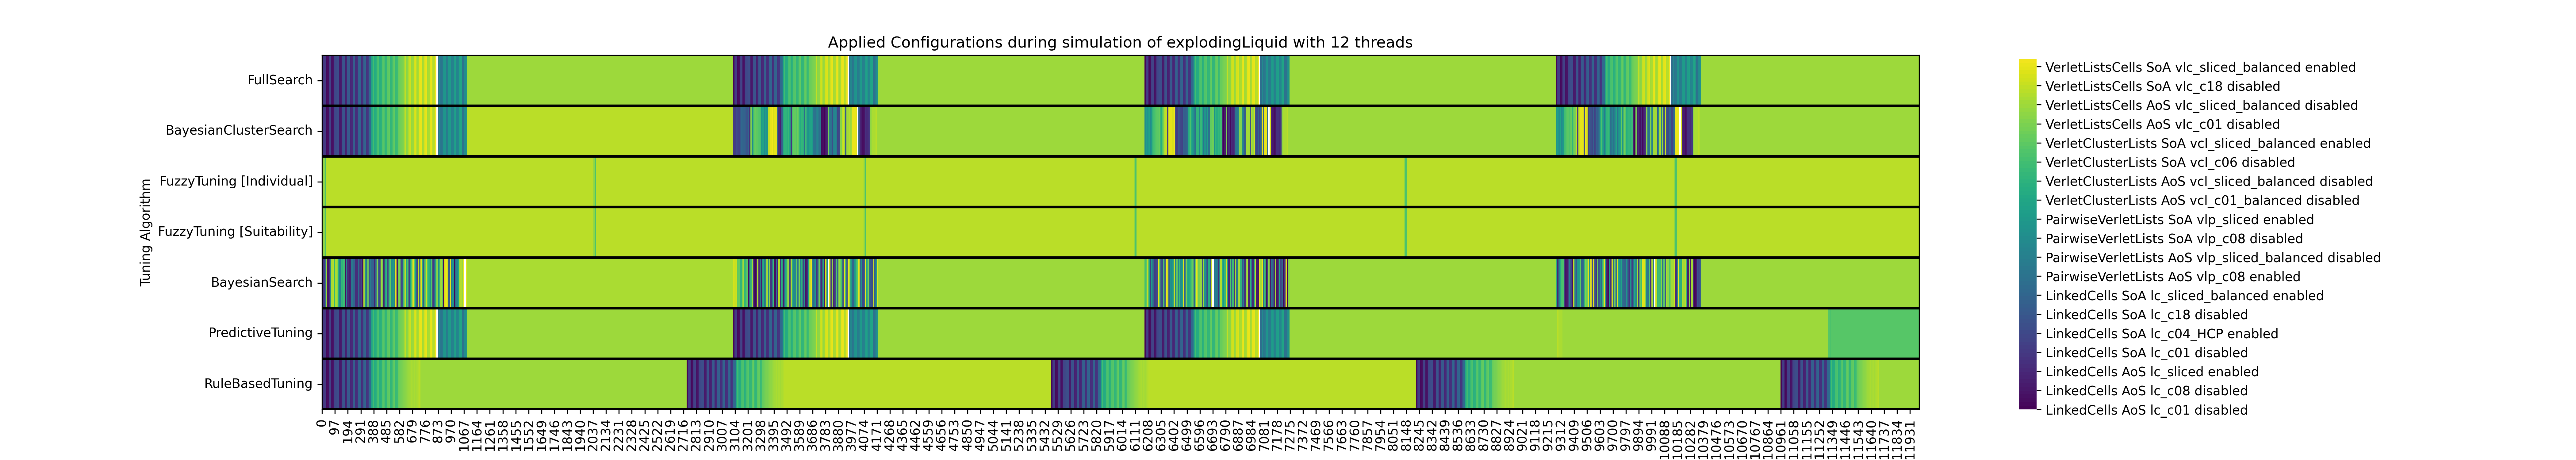
\includegraphics[height=8cm,trim={54cm 0 5cm 0cm},clip]{figures/Benchmark/colorbar_explodingLiquid.png}
  \caption{
      Colorbar for the heatmaps used in the \ref{sec:comparison_and_evaluation} section.
  }
  \label{fig:colorbar_explodingLiquid}
\end{figure}
